\subsection{Terrain Generation}
We will approach this subproblem by first generating a heightmap that represents the hills and the valleys of the landscape. 
A heightmap is a bitmap image where each pixel typically store values representing a surface elevation or displacement.
This is often visualized as a grayscale image where the black pixels represents the minimum height displacement and white the maximum elevation.
To the projects particular use case the pixel values will store the terrain elevation and converted into a 3D mesh. % "converted into 3d mesh" true for Unity Terrain API??
One downside of using a heightmap representation for terrain is its limitation to represent more complex 3D geometry such as caves or overhangs but since the focus of the project is on city generation and not the terrain this is not seen as a problem.
Figure~\ref{fig:heightmap} shows an example heightmap visualized as a grayscale image.

% NOTE(anton): image generated from https://cpetry.github.io/TextureGenerator-Online/
\begin{figure}[h]
  \centering
  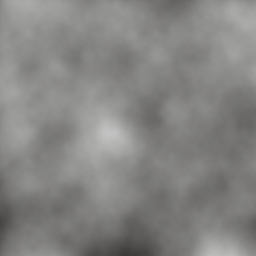
\includegraphics[width=0.25\textwidth]{figure/heightmap.png}
  \caption{An example heightmap generated using Perlin Noise} 
  \label{fig:heightmap}
\end{figure}

We plan to generate the heightmap using multiple layers of simplex noise.
Simplex noise is a type of gradient noise commonly used in computer graphics. 
Gradient noise is one out of two commonly used noises used for terrain generation, the other being value noise.  
The concept of value noise is creating lattice points with pseudorandom values. 
The noise function then returns the interpolated values of the surrounding lattice points. 
Where as gradient noise creates a lattice of pseudorandom gradients, the dot products of the gradients are then interpolated to obtain values between the lattices. 
The user will provide a value for the sea level in the form of a number, and we will color the terrain based on the height levels e.g.\ grasslands near sea level, rocky mountain textures for the taller regions, and snow for top peaks of some of the taller mountains.
The landscape might end up looking something like this, although with less water and mountains, and more flat areas for cities to be placed.

If there is still time after previously mentioned implementations have been made we intend to make the terrain more interesting by generating trees and grass throughout the world.
The way we intend to do this is to use poisson disc sampling to distribute points for trees, and then for grass. % source: https://odr.chalmers.se/handle/20.500.12380/244588
We should sample trees first since they will have a larger radius.  